\chapter{Process Diagnostics: Variation, Flow and Alerts}

\begin{weekbox}
\textbf{Theme.} Before predicting or optimising a process, find out how it actually runs: how variable it is, where
work waits, which cases break the rules, and when a signal is worth a call-out.\\
\textbf{Outcomes.} LO3.\quad \textbf{Tools.} PM4Py (with Graphviz), pandas, scikit-learn.\\
\textbf{Real data.} Receipt phase of a municipal environmental-permit process (1\,434 cases); temperature of an
industrial machine that failed (NAB, 22\,695 readings).\\
\textbf{Lab.} Discover the process map, measure hand-off delays, test conformance rules, verify Little's Law, build a
$p$-chart, and choose an alert rule by its cost.\\
\textbf{Deliverable.} Lab notebook; capstone proposal due at the start of Week 3. \textbf{CA1} follows this week.
\end{weekbox}

\begin{timetable}
0:00--0:20 & Briefing & ``The permit office says it is overloaded. Is it slow everywhere, or at one hand-off?''\\
0:20--1:10 & Concepts & Common vs special cause, control charts, Little's Law, event logs, conformance, alert costs\\
1:10--2:40 & Guided lab & Lab 2, Parts A--C (break at 1:55)\\
2:40--3:40 & Challenge & Exercises 2.3--2.7; capstone proposal in teams\\
3:40--4:00 & Debrief & Which detector would you deploy on the machine, and what would it cost per month?\\
\end{timetable}

\section{Variation: common causes and special causes}
Every process varies. Walter Shewhart's insight at Bell Telephone Laboratories in the 1920s was that variation has two
sources, and that confusing them causes most bad management decisions.

\begin{definition}{Common and special causes}
\emph{Common-cause} variation is the background noise of a stable process: many small causes, always present,
predictable as a distribution. \emph{Special-cause} variation comes from something specific and assignable: a broken
machine, a new clerk, a holiday. A process with only common-cause variation is \emph{in statistical control}.
\end{definition}

The two need opposite responses. A special cause should be found and removed (or kept, if it is good). Common-cause
variation can only be reduced by changing the system: reacting to each point (``Tuesday was slow, hold a meeting'')
adds variation instead of removing it. Deming called this \emph{tampering}.

\subsection{Control charts}
A control chart plots a statistic over time with a centre line and limits at three standard errors. Points outside the
limits, or non-random patterns inside them, signal a special cause.

\begin{keyformula}{Common control charts}
\begin{tabular}{@{}L{3.3cm}L{9.6cm}@{}}
Individuals (I) chart & $\bar x \pm 2.66\,\overline{MR}$, where $\overline{MR}$ is the mean absolute difference between consecutive points\\
$p$-chart (share defective) & $\bar p \pm 3\sqrt{\bar p(1-\bar p)/n_t}$; limits widen when the sample $n_t$ is small\\
$c$-chart (counts) & $\bar c \pm 3\sqrt{\bar c}$\\
EWMA chart & $z_t=\lambda x_t+(1-\lambda)z_{t-1}$, limits $\mu\pm L\sigma\sqrt{\lambda/(2-\lambda)}$; detects small drifts\\
\end{tabular}
\smallskip
Western Electric run rules add signals for patterns: 2 of 3 points beyond $2\sigma$ on one side; 4 of 5 beyond $1\sigma$;
8 in a row on one side of the centre line.
\end{keyformula}

\paragraph{Phase I and Phase II} Limits are estimated on a period believed to be in control (Phase I) and then
\emph{frozen} to monitor new data (Phase II). Limits that keep re-estimating themselves on recent data slowly absorb a
drift and never signal it. Lab 2 shows exactly this failure on a real machine.

\begin{example}{A $p$-chart for late shipments}
A warehouse ships $n=200$ orders a day; over 20 in-control days, 1\,000 of 4\,000 orders left late, so $\bar p=0.25$.
Limits: $0.25\pm3\sqrt{0.25\times0.75/200}=0.25\pm0.092$, i.e.\ $[0.158,\,0.342]$. A day with 62 late orders
($p=0.31$) is inside the limits: common cause, do not hunt for a culprit. A day with 75 ($p=0.375$) is a signal:
investigate that day.
\end{example}

\section{Flow: Little's Law and bottlenecks}
\begin{keyformula}{Little's Law}
For any stable system, average work in process $L$, throughput rate $\lambda$ and average time in system $W$ satisfy
\[ L=\lambda W. \]
It needs no assumption about distributions, order of service or the number of servers.
\end{keyformula}
Little's Law turns any two measurable quantities into the third. If a permit office receives 3.4 cases a day and holds
17 open cases, the average case takes $17/3.4=5$ days. To cut that to 3 days without changing demand, the office must
hold no more than about 10 cases in process: a target a manager can see.

\paragraph{Bottlenecks} Throughput of a serial process is set by its slowest resource (the bottleneck); time added
before the bottleneck is mostly waiting. In event data the bottleneck shows up as the hand-off with the largest
\emph{total} waiting time (frequency $\times$ mean wait), which is not always the slowest single step.

\section{Process mining}
\begin{definition}{Event log}
An event log is a table with at least a \emph{case ID} (which instance: an application, an order), an \emph{activity}
(what happened) and a \emph{timestamp} (when). Resources, costs and case attributes are optional extras. The ordered
sequence of activities of one case is its \emph{trace}; a distinct trace is a \emph{variant}.
\end{definition}

Process mining has three tasks. \textbf{Discovery} builds a model of the real process from the log; the simplest is
the directly-follows graph (DFG), whose arc $a\rightarrow b$ counts how often $b$ immediately follows $a$ in a case.
\textbf{Conformance} compares the log with rules or a reference model and finds deviating cases. \textbf{Enhancement}
adds performance (waiting times, resources) to the model.

\begin{pitfall}{Spaghetti and recording artefacts}
Real logs produce unreadable ``spaghetti'' maps. Filter to the variants covering most cases, then study the rest
separately. And remember that timestamps record when someone \emph{clicked}, not when work happened: a batch of
tasks entered at 16:55 will look like a two-minute process.
\end{pitfall}

\section{Anomaly alerts are decisions}
An alert is a decision rule: \emph{call out a technician when the score exceeds $k$}. Each threshold trades false
alarms against missed events, and the right trade depends only on what each costs.

\begin{keyformula}{Choosing a threshold by cost}
For a detector with threshold $k$, over an evaluation period,
\[ \text{Cost}(k) = c_{\text{FA}}\cdot \text{FA}(k) + c_{\text{miss}}\cdot \text{Miss}(k), \]
and the deployed threshold minimises it. For a single alarm with event probability $p$, it is worth acting when
$p > c_{\text{FA}}/(c_{\text{FA}}+c_{\text{miss}})$.
\end{keyformula}
Precision, recall and F1 weight the two errors arbitrarily; a manager does not. If a missed failure costs 8\,M\xaf\ and
a call-out 150\,000\xaf, it is worth accepting up to 53 false alarms to catch one more failure.

Detectors range from simple to complex: fixed control limits; robust $z$-scores against a moving median and MAD;
model-based scores such as Isolation Forest, which isolates unusual points with random splits. The lab compares all
three on the same labelled failures. Complexity must earn its place.

% ------------------------------------------------------------------ LAB
\section{Practical Lab 2: Diagnosing a permit office and a failing machine}
\begin{labbox}{Practical lab --- real event log and real sensor data}
\textbf{Goal.} Part A: map and measure a municipal process. Part B: monitor its service level with a control chart.
Part C: choose an alert rule for a machine by cost. \textbf{Files.} \texttt{real/receipt.xes},
\texttt{real/machine\_temperature\_system\_failure.csv}, \texttt{real/combined\_windows.json}. \textbf{Time.} 90 minutes.
\end{labbox}

\subsection*{Part A --- Process mining}
\step{Step 1: Load the log and count variants}
\codeout{lab2_s1}{Reading an XES event log with PM4Py and listing the variants.}
\interp{1\,434 applications, but 116 different paths. The ``happy path'' (receipt, T02 check, T04 determine, T05
send confirmation, T06 and T10 stop-advice checks) covers half the cases; the top five cover 80\%. 116 cases (8\%)
stop after the receipt is registered: they never get a confirmation.}

\step{Step 2: Discover the process map}
\codeout{lab2_s2}{Directly-follows graph of the eight most common variants.}
\begin{figure}[H]\centering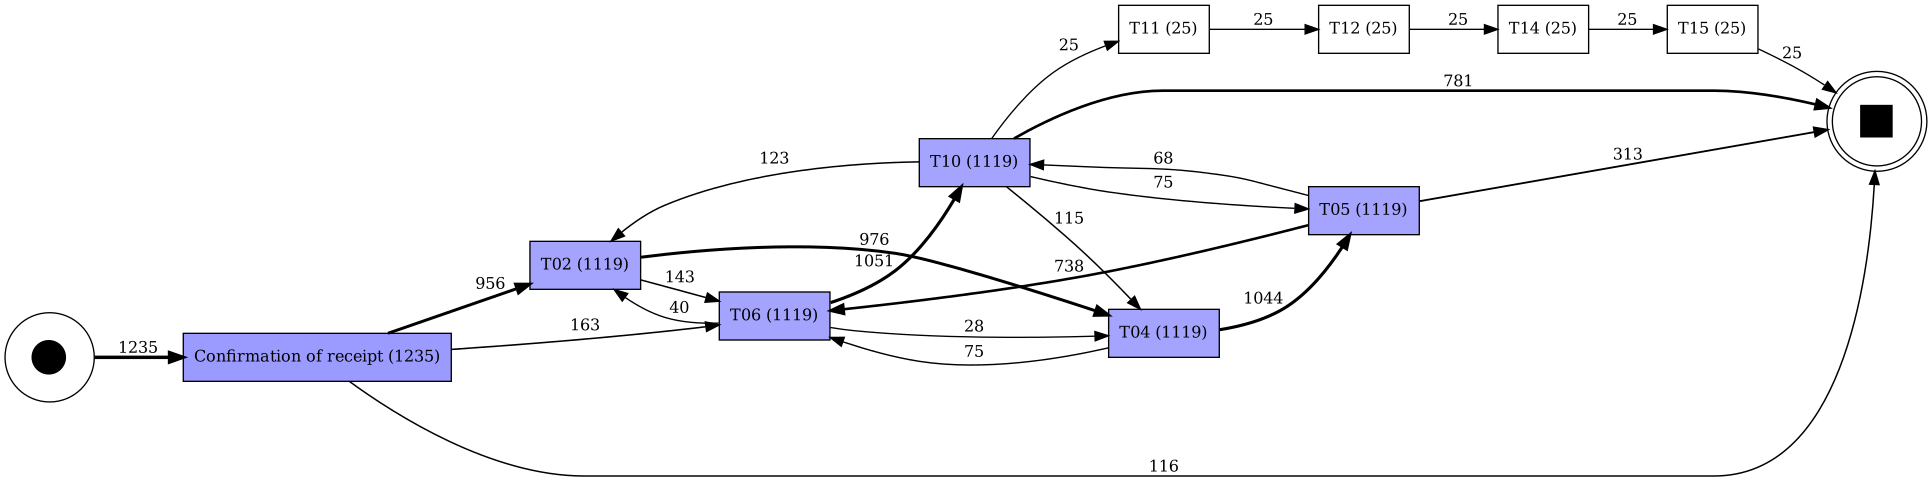
\includegraphics[width=\linewidth]{../figs/lab2_dfg.png}
\caption{Directly-follows graph (counts) of the main variants of the receipt process.}\end{figure}
\interp{The map shows two orderings: T02--T04--T05 first, then T06--T10, or the reverse. The office does not follow one
sequence, which is not necessarily wrong but is worth asking about: does the order change the outcome?}

\step{Step 3: Where does time go?}
\codeout{lab2_s3}{Case durations and waiting time per hand-off.}
\interp{The median case is closed in 0.03 days (45 minutes): most applications are handled in one sitting. But the
mean is 5.4 days and the slowest 10\% take over two weeks, so the \emph{tail} is the problem, not the typical case. The
hand-off from T05 (send confirmation) to T06 (stop-advice check) has a median wait of zero yet accounts for 2\,422
case-days of waiting: a few cases wait there for weeks. That is where to look first.}

\step{Step 4: Conformance rules and deadlines}
\codeout{lab2_s4}{Declarative rules checked case by case, and their link to lateness.}
\interp{The ordering rules always hold; the problems are cases that never reach T05 (9.3\%) and cases where a task
repeats (6.3\%). Non-conforming cases miss their deadline 16.4\% of the time, against 4.6\% for conforming ones:
conformance is not bureaucracy here, it predicts lateness.}

\step{Step 5: Check Little's Law}
\codeout{lab2_s5}{Arrival rate times time in system versus measured work in process.}
\interp{$\lambda W=16.8$ against a measured average of 17.4 open cases: the law holds on real data to within 4\%,
the gap being start and end effects of the window. The office could set a WIP limit of about 10 cases to bring the
average to 3 days, provided it clears the long-waiting tail rather than starting new cases faster.}

\subsection*{Part B --- Monitoring the service level}
\step{Step 6: A $p$-chart of slow cases}
\codeout{lab2_s6}{Weekly share of cases taking more than seven days, with variable control limits.}
\begin{figure}[H]\centering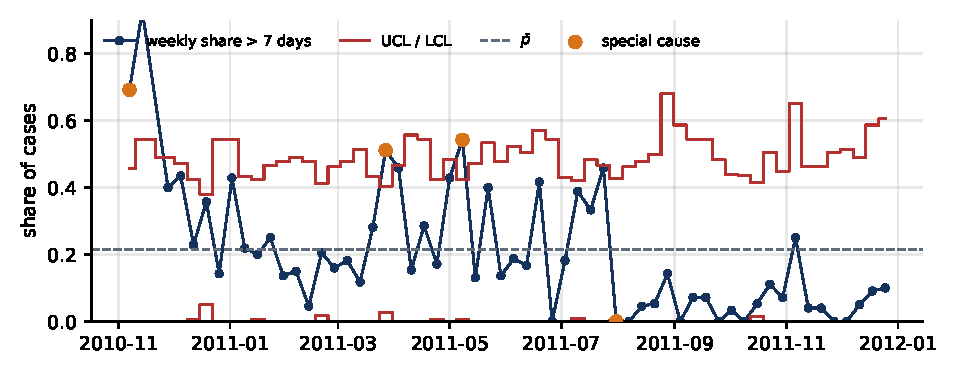
\includegraphics[width=0.92\linewidth]{../figs/lab2_pchart.pdf}
\caption{$p$-chart of the weekly share of cases slower than 7 days. Limits widen in weeks with few cases.}\end{figure}
\interp{About one case in five takes more than a week. The two signals in November 2010 belong to the start-up period
of the log and would be removed from Phase I. Late March and early May 2011 are genuine special causes worth asking
about (holidays, staff absence, a batch of complex applications). The week of 31 July with \emph{no} slow cases is
also a signal: find out what went right.}

\subsection*{Part C --- An alert rule for a failing machine}
\step{Step 7: Two detectors, judged by cost}
\codeout{lab2_s7}{Adaptive robust $z$-score versus fixed Phase I limits on a moving average.}
\begin{figure}[H]\centering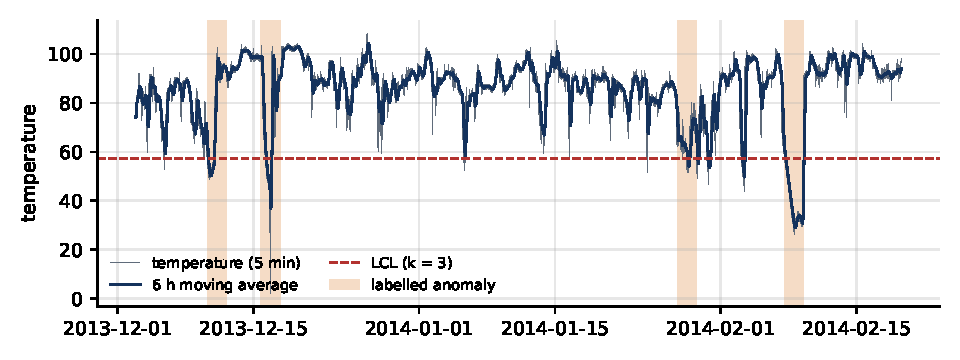
\includegraphics[width=0.92\linewidth]{../figs/lab2_nab.pdf}
\caption{Machine temperature, its 6-hour moving average, the Phase I lower limit and the four labelled anomalies
(shaded), the third being a catastrophic failure.}\end{figure}
\interp{The adaptive detector never catches all four events at any threshold: its 24-hour baseline drifts down with
the machine and absorbs the slow degradation before the failure. The fixed-limit chart on the 6-hour average catches
all four with three false alarms at $k=3$, an expected cost of 0.45\,M\xaf\ against at least 8.75\,M\xaf\ for the
adaptive rule. Raising $k$ to 3.5 looks ``cleaner'' (one false alarm) but misses a failure, which is twenty times
worse.}

\step{Step 8: Does a machine-learning detector do better?}
\codeout{lab2_s8}{Isolation Forest trained on the Phase I week, thresholded by score quantile.}
\interp{Isolation Forest also catches all four events, but only at a loose threshold with 23 false alarms
(3.45\,M\xaf). On this machine a well-designed control chart is cheaper, simpler to explain to a maintenance crew, and
needs no retraining. Model-based detectors earn their place with many interacting sensors, where a single chart
cannot see the pattern.}

\paragraph{So what (model answer)} \emph{Half of all permit applications follow one path and are closed within the
hour; the problem is a tail of cases that wait weeks between sending the confirmation and the stop-advice check, and
cases that never get a confirmation, which are three times as likely to miss their deadline. For the machine, a
moving-average chart with limits fixed on a healthy week would have flagged all four incidents, including the failure,
for about 0.45\,M\xaf\ of call-outs.}

% ------------------------------------------------------------------ EXERCISES
\section{Exercises}
\begin{enumerate}[label=\textbf{2.\arabic*},leftmargin=2.4em]
\item \emph{(Concept)} A manager reviews the daily late-order count and calls a meeting whenever it rises above
yesterday's. Explain, with the language of common and special causes, why this makes things worse.
\item \emph{(Calculation)} A clinic sees 40 patients an hour, each spends on average 54 minutes from arrival to
departure. How many patients are inside on average? If the waiting room seats 30, what must happen to the time in
system?
\item \emph{(Control chart)} For the Mboa clinic (\texttt{clinic.csv}), compute the daily mean service time and draw an
I-chart. Are any days out of control? Apply the Western Electric rules.
\item \emph{(Process mining, Mboa)} Using \texttt{event\_log.csv}, find the variants, the rework rate on ``Documents
Check'' and the hand-off with the largest total waiting time. Is Monday different?
\item \emph{(Conformance)} The registration office states the rule ``no enrolment before fee payment''. What share of
cases violate it, and does violation predict a longer cycle time?
\item \emph{(Alert cost)} Repeat Step 7 with $c_{\text{FA}}=400\,000$\xaf\ (the technician travels from Douala). Does the
chosen threshold change? At what false-alarm cost would $k=3.5$ become optimal?
\item \emph{(Phase I)} Re-estimate the Phase I limits on the second week instead of the first. How sensitive is the
result? Write two sentences on how you would choose a Phase I period on a new machine.
\end{enumerate}

\section{Take-home assignment 2 and capstone proposal}
\begin{enumerate}[nosep]
\item Write a two-page diagnosis of the receipt process for the head of the permit office: the three findings that
matter most, each with a number, and one recommended change with its expected effect on lateness.
\item \textbf{Capstone proposal} (one page, due start of Week 3): the decision statement, the dataset and its owner,
the KPI and both error costs, the baseline policy you will try to beat, and the methods you expect to use.
\end{enumerate}
\paragraph{CA1 preparation} CA1 gives you an unseen transaction file and event log. You will audit, compute KPIs,
diagnose one process and write a manager summary in two hours. Practise on the Mboa files.
